%%%%%%%%%%%%%%%%%%%%%%%%%%%%%%%%%%%%%%%%%%%%%%%%%%%%%%%%%%%%%%%%%%%%%%%%%%%%%%%%
%2345678901234567890123456789012345678901234567890123456789012345678901234567890
%        1         2         3         4         5         6         7         8
% THESIS CHAPTER

\chapter{Experimental measurements and metodology}
\label{chap:ex}
\ifpdf
    \graphicspath{{Chapter4/Figures/PNG/}{Chapter3/Figures/PDF/}{Chapter4/Figures/}}
\else
    \graphicspath{{Chapter4/Figures/EPS/}{Chapter3/Figures/}}
\fi


% short summary of the chapter
\section*{Summary}
In this chapter the metodology followed in experiments and the different measuremns 
that are observed during the data transmission are explained in detail.

\section{Measurements} 
\label{chap4:meas}

The following indicators describe the quality of our wireless LoRaWan communication 
in the mentiened experiments:

\subsection{RSSI}
\label{chap4:rssi}

\acrfull{rssi} is one indicator that provides the information 
about how strong the received signal is. It is masured in dBm and its value 
is always below zero, this means that the closer to zero the RRSI value, the stronger 
the received signal is.\\
This indicator is calculated by the sum of different paramenters like the path loss, 
the transmission power of the antenna, the cable losses and the antenna gain.

\subsection{SNR}
\label{chap4:snr}

This indicator of quality of signal received takes into account the noise floor signal power in the 
comunnication. When we transmit in wireless comunnication, the presence of the noise can surpass 
the power of signal received and not being able to get any information from the signal. The \acrfull{snr} is 
also measured in dBm and it's the subtraction between the power received and the power of the 
noise floor during the comunnication.\\
However, LoRa due to its demodulation explained in chapter 2, is able to demodulate 
and extract information from the signal for negative SNR values. The limit of the minimun 
value of SNR for the receiver depends on the SF as the figure below shows:

\begin{table}[htbp]
    \centering
    \setlength{\arrayrulewidth}{0.5mm}
    \setlength{\tabcolsep}{18pt}
    \renewcommand{\arraystretch}{2}
    \begin{tabular}{|c|c|c|}
        \hline
         \cellcolor[HTML]{85C1E9}SF & \cellcolor[HTML]{85C1E9}chips / symbol & \cellcolor[HTML]{85C1E9}SNR limit\\
         \hline
         SF7 & 128 & -7.5 dB\\
         SF8 & 256 & -10 dB\\
         SF9 & 512 & -12.5 dB\\
         SF10 & 1024 & -15 dB\\
         SF11 & 2048 & -17.5 dB\\
         SF12 & 4084 & -20 dB\\
         \hline
    \end{tabular}
    \caption{Limit SNR and chips per symbol for different SF}
    \label{tab:my_label}
\end{table}

\subsection{Packet Loss}
\label{chap4:packloss}

The Packet Loss is simply the ratio between the packets that the 
gateway is receiving and the packets the end node is sending.
This measure is observed thanks to the frame counter that the LoRa packets implent. 
The frame counter contains the number of packets that the end node is sending.\\
In order to calculate this ratio the frame counter and the number of packets that 
appear in our TTN server are considered.

\section{Metodology}
\label{chap4:metod}

\subsection{First Experiment}
\label{chap4:exp1}

The ADR as it's introduced in \ref{sec:f-ttnandlora} can modify parameters of communication 
such as the SF, the transmission power or the BW to get a better SNR or to 
reduce the excesive power consumption of the end node.\\

The so-called “Margin” is calculated after a number of transmissions (uplink).
The maximun SNR of those transmissions minus the required SNR to demodulate a 
message given the data rate are considered. This margin is used to determine 
how much we can increase the data rate or decrease the transmit power.\\

In the things stack for modifying the SF to increase the SNR and get a better communication, 
64 packets without a downlink message of the ADR are needed. In that case the node will 
increase the SF or the transmission power in order to start receiving downlink packets again.\\

In the case that the margin is high enaugh, which means that the node is consuming excessive power, 
the ADR after 20 packets of uplink sends a dowlink message to the node in order to adapt the 
parameters of comunnication and consume less power.\\

As it can be supossed from the last information about the ADR, its performance is usefull 
when the end node is fixed. But if the end node is moving with the ADR activated, 
what happens to the comunnication? Is better for the data transission to fix one 
SF and the transmission power in the end node?\\

Those questions were formulated in order to perform our first experiment.\\
In this first experiment two types of configuration between the end node and the TTN servers are selected. 
In one, the ADR is activated from both sides of the comunnication as it follows:

\begin{figure}[htbp]
    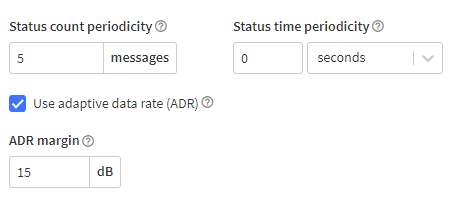
\includegraphics[width=\linewidth]{ADR_config}
    \caption{ADR configuration in TTN console}
\end{figure}

For the other one a medium SF is selected, SF10, and the transmission power is fixed to the default one (14 dBm).\\
The idea of this experiment is to follow the same route in a urban area for both configurations and analize 
which is performing better by measuring the packet loss, RSSI and SNR in both cases. 
The route planned for this experiment is inside the city of Genova, in the Porto Antico area as it is 
ilustrated in \vref{chap4:genovaRoute}

\begin{figure}[htbp]
    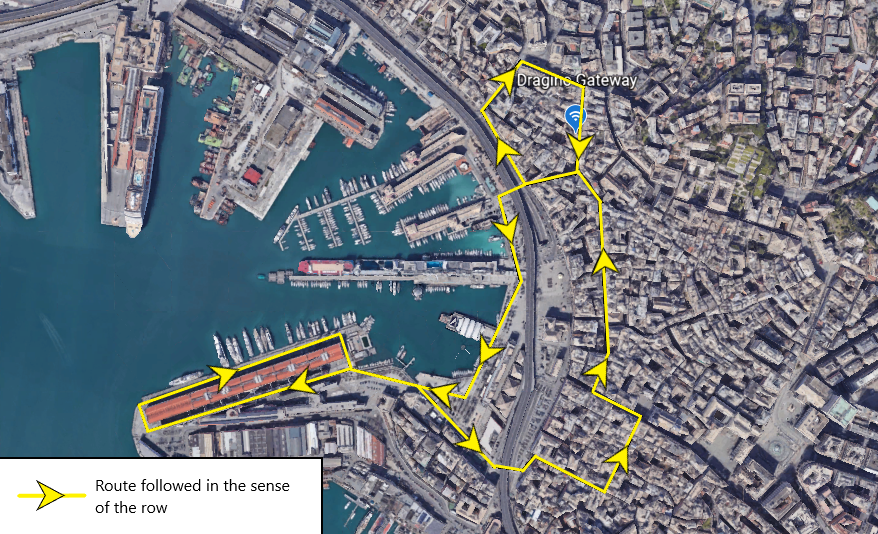
\includegraphics[width=\linewidth]{Gnv_route.png}
    \caption{Area of Genova where the experiment is performed}
    \label{chap4:genovaRoute}
\end{figure}

Thanks to a battery connected to the adafruit board the mobile end node is builded. 
This battery was attached to the bottom of the board and packed inside a tupper as it is ilustarated 
in \ref{chap4:endNode0} allowing us to move confortably following the planned route.

\begin{figure}[htbp]
    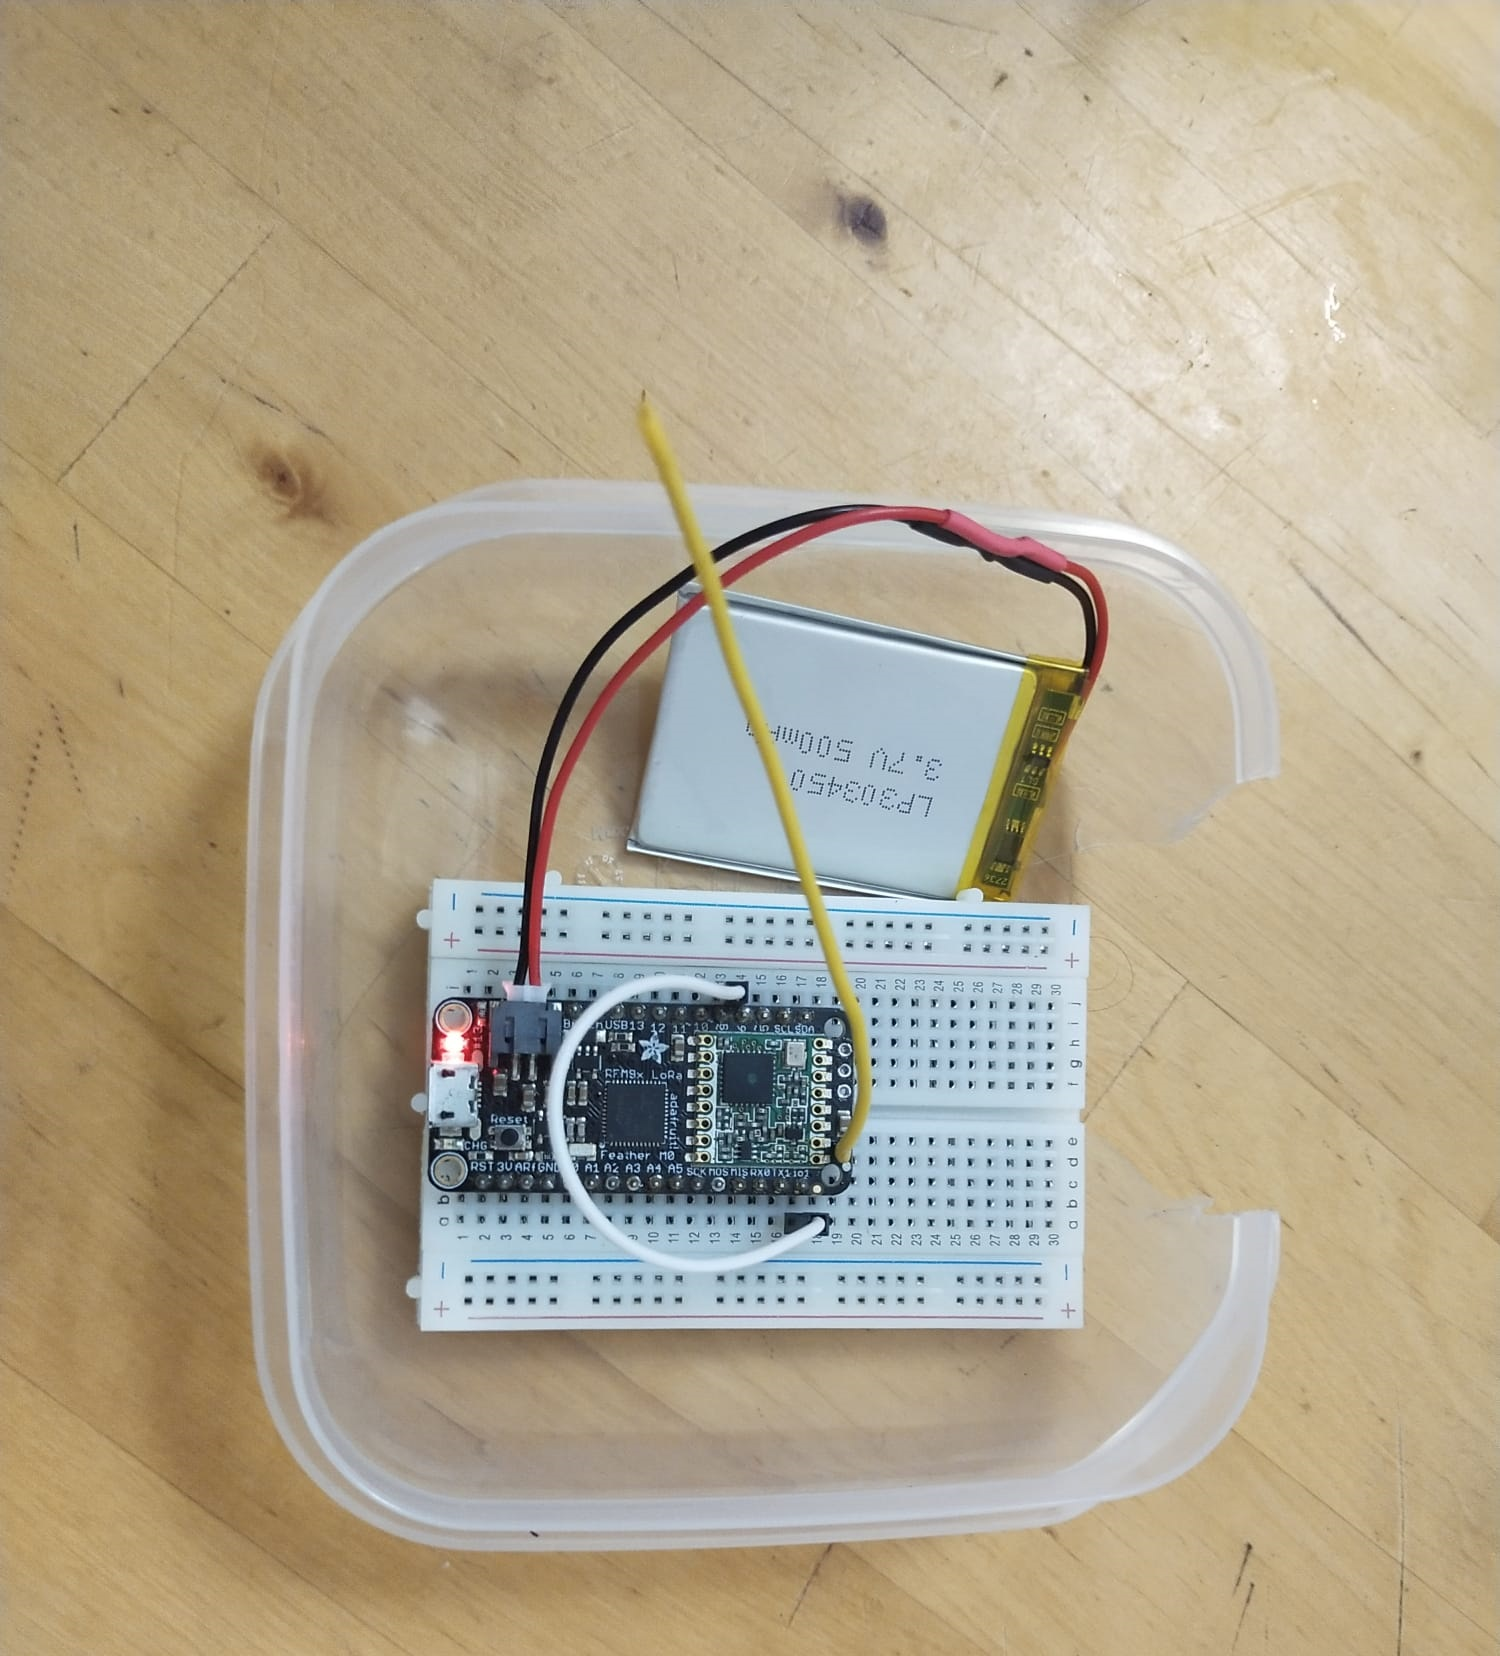
\includegraphics[width=\linewidth]{EndNode0.jpeg}
    \caption{LoRaWan mobile end-node used}
    \label{chap4:endNode0}
\end{figure}

\subsection{Second experiment}
\label{chap4:exp2}

The ADR shows how important is to choose the correct \acrfull{tx power} and SF in a LoRaWan data transmission. The margin 
calculated by the network server depends basically on how far from the gateway the ED is located and on the 
area/landscape the network is placed. We know that different scenarios can cause a huge difference in terms 
of interference for our comunnication, e.g, in an open space LoRaWan protocol is able to perform much better 
than in urban areas where buildings and other causes of interference are present. This idea is corroborated 
by the thesis (link).

We wanted to know how different transmission parameters can affect a LoRaWan communication without the use of ADR
and to see the infuence of different landscapes inside a urban area for the indicators cited in \ref{chap4:meas}.

The idea for this second experiment the objective is to further expand and analyze the results obtained previously 
designing a program that will be running in the adafruit board that is constantly changing the values of SF and Tx power. 


Once the device is set up we modified our test code to send the coordinates of its current position 
which will allow us to calculate te distance from our Gateway to the end node and it also allows us 
to trace the path and determine in which part of the city we are sending our packages. With this 
information we can analyze how different parameters behave in different enviroments.

The area of testing will be the same as in the last esperiment with the exception that in this experiment
we won't follow a fixed route.
